\subsection{Comparison with PDEVS}
In this section we contrast the speedup between the original PDEVS algorithm and the synchronization protocols. 
Note that the PDEVS algorithm and the synchronization protocols are complementary in \textit{dxex}, not exclusive. 
Following the theoretical analysis published in ~\cite{amdahlpdevs} a comparison between PDEVS and the synchronization protocols was warranted. 
We compare the ideal scenario for PDEVS where all events are concurrent with a scenario where events are random.
In this work we do not consider the distribution of events, introducing a random number generator as we will show in this work can mask performance results. 
By limiting ourselves to the best and worst case scenario we demonstrate the capabilities and limitations of both approaches.
The influence of the computational load of the transition functions is a second factor we investigate in this section.
We are interested in scenarios where PDEVS and the synchronization protocols can complement each other in addition to observing their speedup in isolation.
The benchmarks are run on the same hardware as our previous results, a 8 x AMD Opteron(TM) Processor 6274 machine with 8 cores per cpu (64 cores) and 192 GB RAM. 
The benchmarks use a maximum of 16 threads to be divided between PDEVS , conservative or optimistic. 

\paragraph{Model}
As shown in the previous section, when most models are dependent on each other across kernels there is no speedup obtainable by either optimistic or conservative. 
We therefore opted to use the \textit{Queue} model in this benchmark, with depth 4 and width 300.
The effect of combining 4 synchronized kernels with each 4 threads for PDEVS is contrasted with 16 threads for PDEVS and 16 kernels for conservative and optimistic.  
This allows us to observe which is more efficient in obtaining a speedup.
We simulate a computational load by a call to sleep in the transition functions set at 5ms. 

\paragraph{Concurrent events}
First we create the ideal scenario for PDEVS, all events are concurrent with a significant computational load in the transition functions. 

In figure \ref{fig:pdevs_plot_fixed_sleep} we observe that PDEVS obtains a speedup approaching 8. 
Conservative and optimistic are run first with 16 kernels, then with 4 kernels having 4  PDEVS threads each. 
The resulting speedup is half of that obtained of the sequential kernel with 16 PDEVS threads.

\paragraph{Random events}
Random events allow us to demonstrate the overhead of PDEVS. The probability that events are concurrent is strongly reduced.
The transition function has the same computational load as in the previous configuration. 
The results in figure \ref{fig:pdevs_plot_random_sleep} demonstrate that the overhead in the sequential DPEVS kernel is negligible. In contrast both conservative and optimistic suffer a significant slowdown when combined with PDEVS.
We clearly see that conservative and optimistic outperform the sequential kernels in this scenario, complementing the synchronized kernels with PDEVS is not warranted here.

\paragraph{Computational load}
When we remove the computational load we isolate the overhead of the parallelism. 
In this paper we are mainly interested in this overhead which is otherwise masked by adding a computational cost to the transition functions. 
All the benchmarks in this work are run with a near negligible computational load in the transition functions for this purpose.
If a parallel speedup can be obtained in a simulation model without any load in the transition function this will translate in a higher speedup with an increased load, as this load can then be spread over kernels or threads.
Although this configuration has only concurrent events the overhead of the synchronization is severe. 
The runtime cost of this overhead is extreme in the sequential kernel. 
The synchronized kernels are impacted less by the overhead of the PDEVS algorithm.
 
\paragraph{Discussion}
In \textit{dxex} PDEVS and the two synchronization protocols are complementary. The user is not forced to choose between either but can divide the capabilities of his machine over both approaches.
While PDEVS can offer a significant speedup we see that to offer this speedup the concurrency of events must be significant in combination with a high computational load in the transition functions. 
We measure the overhead introduced by PDEVS to give practitioners insight into which model can benefit from which paradigm.
The overhead of the synchronization protocols in specific scenarios  is shown in the previous section.
For a given model it is difficult to predict the concurrency of events, although the computational load of a transition function can be approximated.
In these benchmarks we show which configurations can lead to a speedup for PDEVS or the synchronization protocols in isolation or combination.


\begin{figure}
	\center
	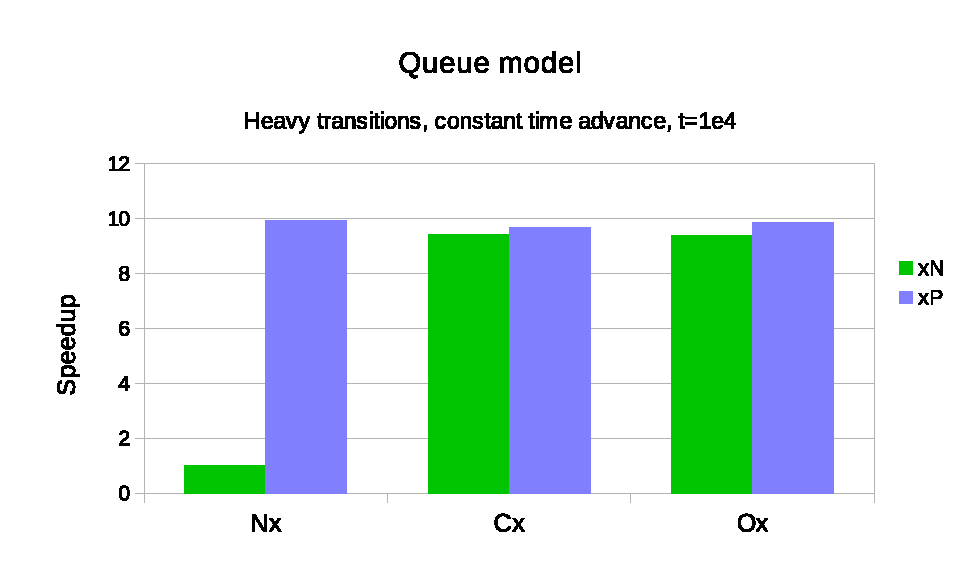
\includegraphics[width=\columnwidth]{fig/pdevs_fixed_sleep.eps}
	\caption{Queue speedup benchmark for PDEVS and synchronization with maximal concurrent events and significant computational load}
	\label{fig:pdevs_plot_fixed_sleep}
\end{figure}

\begin{figure}
	\center
	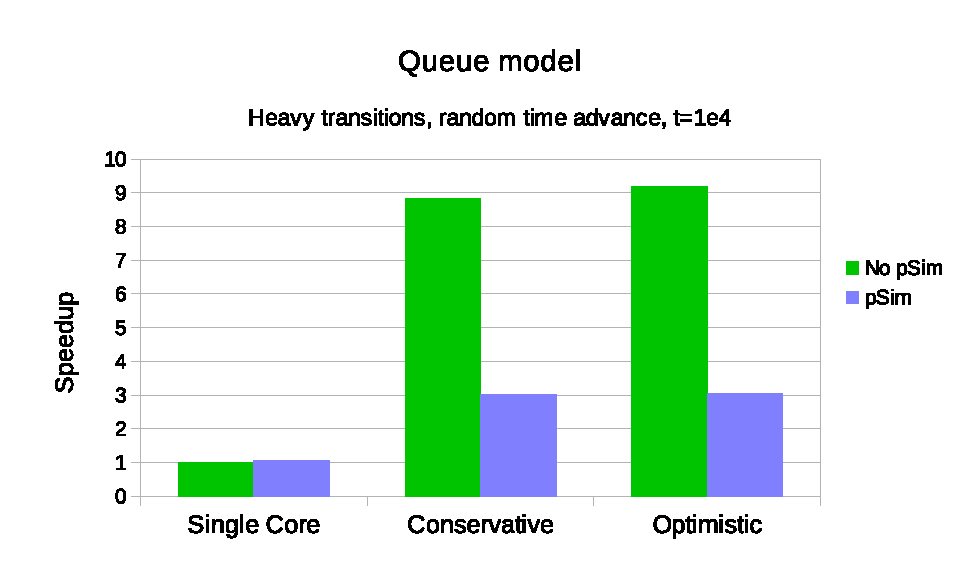
\includegraphics[width=\columnwidth]{fig/pdevs_random_sleep.eps}
	\caption{Queue speedup benchmark for PDEVS and synchronization with randomized events and significant computational load}
	\label{fig:pdevs_plot_random_sleep}
\end{figure}

\begin{figure}
	\center
	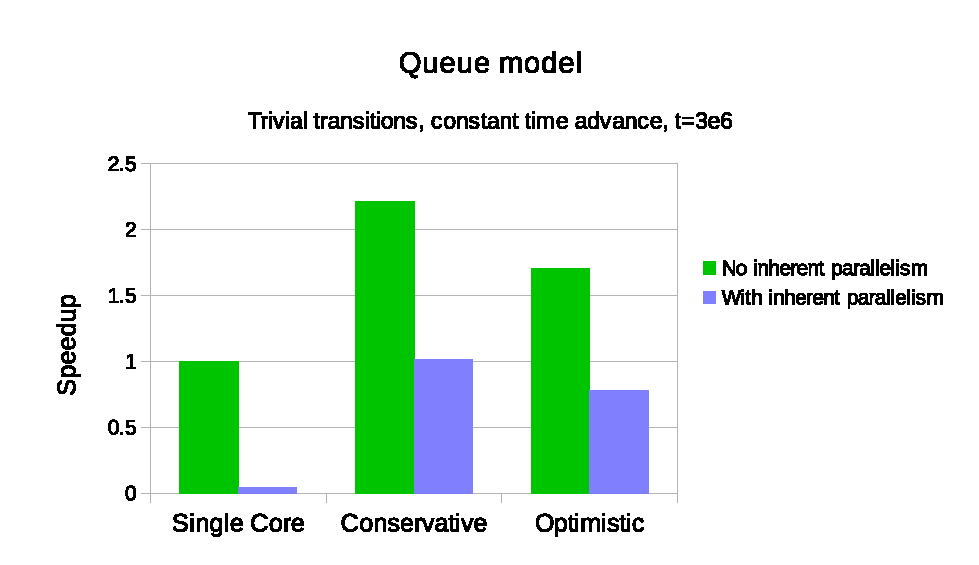
\includegraphics[width=\columnwidth]{fig/pdevs_no_sleep.eps}
	\caption{Queue speedup benchmark for PDEVS and synchronization with maximal concurrent events and trivial computational load}
	\label{fig:pdevs_plot_no_sleep}
\end{figure} 